\section{Introduction}
	As the adoption rate of battery powered cars increases, the need for a better and more complex route planing solution appears. Battery powered vehicles generally have a shorter range as well as a significantly slower refuel time, compared to traditional gasoline cars. As the refuel time have become a significant factor in the combined travel time, the time spend refueling should be taken into account by a route plan, to accommodate for an otherwise large margin of error.
	Time spend recharging batteries is inherently variable, as the charge rate is significantly affected by both the charge station’s charge rate, as well as the battery’s current charge. When planing a route for a modern electric vehicle, it is therefore paramount to be able to incorporate charge stations, charge rates and battery charge into the plan.
	Another important aspect is resource consumption itself. With the now significant time spend refueling, a high rate of energy consumption while driving, can in turn result in a significant time spend on refueling.
	It should be clear that no traditional shortest path algorithm is able to accommodate for the variables and relationships between travel speed, charge rate and route planing. In this article we present two different approaches to solving the problem of optimizing a route plan for electiv verhicles. One is a linear program..... The other is a more naive solution which uses heuritics..... Both approaches are analysed on accuracy and running speed, based on a real world road network as input.

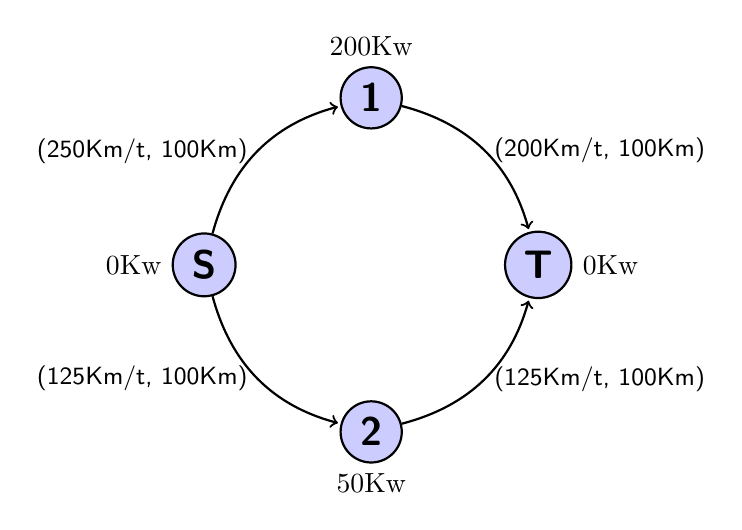
\begin{tikzpicture}[->,->,shorten >=1pt,auto,node distance=3cm,
  thick,main node/.style={circle,fill=blue!20,draw,font=\sffamily\Large\bfseries}]
%1
  \node[main node] (1) {1};
  \node[above] at (1.north) {200Kw};
%2 
 \node[main node] (2) [below left of=1] {S};
  \node[left] at (2.west) {0Kw};
%3 
 \node[main node] (3) [below right of=2] {2};
  \node[below] at (3.south) {50Kw};
%4 
 \node[main node] (4) [below right of=1] {T};
  \node[right] at (4.east) {0Kw};
%paths
  \path[every node/.style={font=\sffamily\small}]
    (1)
	  edge [bend left] node[right] {(200Km/t, 100Km)} (4)
    (2) edge [bend right] node[left] {(125Km/t, 100Km)} (3)
    	  edge [bend left] node[left] {(250Km/t, 100Km)} (1)
    (3) edge [bend right] node[right] {(125Km/t, 100Km)} (4)
    (4) ;
\end{tikzpicture}
